%= local definitions of macros ============================
\newcommand{\Herwig}{H\protect\scalebox{0.8}{ERWIG}\xspace}
\newcommand{\Pythia}{P\protect\scalebox{0.8}{YTHIA}\xspace}
\newcommand{\Sherpa}{S\protect\scalebox{0.8}{HERPA}\xspace}
\newcommand{\Rivet}{R\protect\scalebox{0.8}{IVET}\xspace}
\newcommand{\Professor}{P\protect\scalebox{0.8}{ROFESSOR}\xspace}
\newcommand{\eps}{\varepsilon}
\newcommand{\mc}[1]{\mathcal{#1}}
\newcommand{\mr}[1]{\mathrm{#1}}
\newcommand{\mb}[1]{\mathbb{#1}}
\newcommand{\tm}[1]{\scalebox{0.95}{$#1$}}
\newcommand{\SMEFTsim}{\texttt{SMEFTsim}}
\newcommand{\SMEFTatNLO}{\texttt{SMEFT@NLO}}
\newcommand{\Madgraph}{M\protect\scalebox{0.8}{ADGRAPH}\xspace}
%= title + authors =====================================
\section{Study of EFT effects in loop induced Higgs processes ~\protect\footnote{
  A.~Cueto,
  S.~Pigazzini}{}}

%= MANDATORY label ======================================
\label{sec:projname}

%= (optional) preamble ================================== 
%\begin{abstract}

%\end{abstract}

%= content ===== ========================================
\subsection{Introduction}
\label{sec:higgseft:section1}
The Standard Model Effective Field Theory (SMEFT) approach is a powerful tool to look for hints of new physics. It allows to study large sets of experimental data without assuming that the theory used is valid to arbitrarily high energies. In the SMEFT, the Standard Model (SM) as we know it is just an effective theory at energies around the electroweak scale. Beyond the Standard Model (BSM) physics manifests at higher scales, $\Lambda$, and is parameterised in terms of higher-dimmensional operators that conserve the same fields and symmetries as the SM. At any mass dimension, a complete bases of non-reduntant operators can be worked out and the full Lagrangian can be written as a power expansion
\begin{equation}
\mathcal{L}_{\textrm SMEFT} = \mathcal{L}_{\textrm SM} + \sum_{d>4}\sum_{i}\frac{c_i}{\Lambda^{d-4}}\mathcal{O}_{i}^{(d}),
\end{equation}  

where $\mathcal{L}_{\textrm SM}$ is the SM Lagrangian, $c_i$ are the Wilson coefficients and ${\mathcal{O}^{d}}$ the set of independent operators for dimension $d$. Operators with $d=5,7$  violate lepton and/or baryon number conservation~\cite{Degrande:2012wf,Kobach:2016ami}. Thus, dimension-6 operators represent the leading deviation from the SM and will be the focus of this work. The modification of a cross section by the insertion of one dimesion-6 operator in the amplitudes can be written as

\begin{equation}
\sigma = \sigma_{\textrm SM} + \sum_{i}\sigma_i^{\textrm int} \frac{c_i}{\Lambda^{2}} + \sum_{i,j}\sigma_{(i,j)}^{\textrm BSM} \frac{c_ic_j}{\Lambda^{4}} ,
\end{equation}  

where $\sigma_{\textrm SM}$ is the SM cross section of a given process, $\sigma_i^{\textrm int}$ is the interference between the SM and the BSM amplitudes and $\sigma_{(i,j)}^{\textrm BSM}$ represents the pure BSM correction to the SM cross section. The leading term is formally $\sigma_i^{\textrm int}$ and the one than will be investigated in this work. 

Several bases of independent operators can be found in the literature~\cite{Grzadkowski:2010es,Contino:2013kra,Gupta:2014rxa,Masso:2014xra}. In the context of the study of the Higgs boson, the SILH basis~\cite{Contino:2013kra} has been commonly used. However, it is not optimised for, for example, diboson processes. Even if the translation between bases is known and has been automated~\cite{Falkowski:2015wza,Aebischer:2017ugx}, experimental collaboration have started to publish their EFT interpretations in the Warsaw basis also in the Higgs sector~\cite{ATLAS:2019jst,ATL-PHYS-PUB-2019-042} to facilitate future global fits of electroweak, Higgs and top data.

The procedure to test the EFT effects for a given set of measurements can be tedious in practice and a big effort has been devoted to develop public code to perform this task in a automatic and generic way~\cite{Brivio:2019irc}. For the Warsaw basis, different Universal FeynRules Output (UFO)~\cite{Degrande:2011ua} models are available which can be interfaced with modern event generators.

The \SMEFTsim\ code~\cite{Brivio:2017btx} is a well documented UFO implementation of the full set of dimension-6 operators in the Warsaw basis. Its main scope is the estimation of the leading SMEFT corrections to the SM. The effective Lagrangian is truncated at $\Lambda^{-2}$ and not supported for next-to-leading-order (NLO) simulations. For Higgs data interpretation the model have become of common use due to its completeness~\cite{Ellis:2018gqa,ATLAS:2019jst}.  To reproduce all the main Higgs production and decay channels in the SM, the loop-induced processes ($hgg$, $h\gamma\gamma$,$hZ\gamma$) are included as effective vertices. However, this implementation might not result satisfactory for reasons as the ones exposed below:
\begin{itemize}
\item Only operators with the same point-like structure as the effective vertices included to reproduce loop-induced processes can modify the cross sections of these processes. That means that, for example, a modification of the top Yukawa will not affect the gluoon-gluon fusion process.
\item Given the truncation of the Lagrangian, operators that enter in the shifts to input parameters and that will modify the cross section of any tree-level process does not modify the cross section of loop-induced processes.
\item A reliable computation of the Higgs plus jet  production in gluon-gluon fusion requires top quark loop amplitudes at high $p_{\textrm T}$ and the implementation of $gggH$ vertices.
\item The $gg\to ZH$ process cannot be simulated.
\end{itemize}

To overcome these concerns the \SMEFTatNLO\ tool~\cite{SMEFTNLO} can be used for the loop induced Higgs processes. The tool includes a complete implemation of the SMEFT compatible with NLO QCD predictions. In this work, we study the $gg\to ZH$ and $gg\to H$ processes using this tool. 







\subsection{Comparison between models}
\label{sec:higgseft:section2}
The \SMEFTsim and \SMEFTatNLO tools have been validated against each other~\cite{Durieux:2019lnv}. In this section we compare both models at leading order (LO) by checking the cross sections of the $pp\to ZH$ and $pp\to t\bar{t}H$ processes. The comparison is made at the cross section level and, thus, not expected to be in perfect agreement since it will be affected by phase-space integration. The main goal of this comparison is to show the mapping between the different Wilson coefficients naming and to ensure that the setup used for both models is consistent.

For both models we use the $m_Z$, $m_W$, $G_F$ scheme of electroweak parameters\footnote{We use the \texttt{SMEFTsim\_A\_U35\_MwScheme\_UFO} model for \SMEFTsim and the \texttt{SMEFTatNLO\_U2\_2\_U3\_3\_cG\_4F\_LO\_UFO-LO} model for \SMEFTatNLO}. The \Madgraph 2.6.6 generator is used to obtain the cross sections results. The definition of the processes is as follows for the SM results:

\noindent
{\bf ttH:}\\
\noindent
  \texttt{ define p = p b b$\sim$ }\\
  \texttt{ generate p p $>$ h t t$\sim$ SMHLOOP=0 NP=0 }

\noindent
{\bf ZH:}\\
  \noindent
  \texttt{ define p = p b b$\sim$} \\
  \texttt{ generate p p $>$ h l+ l- SMHLOOP=0  NP=0     }\\
  
  The values of several parameters like $m_W$, $mt$, $\alpha_S$ or $\Gamma H$ differ in the default settings of the models and they were set to the same values.

  The tables below show the comparison between the predictions obtained for SM in both models as well as the interference terms, obtained with the NP$^{\wedge}$2$==$1 (NP$^{\wedge}$2$==$2)  for the SMEFTsim (SMEFTatNLO) model.

\begin{center}
  \begin{table}[h]
    \begin{tabular}{|l|l|c|c|}
      \hline
      \textbf{Operator} &\textbf{W. coefficient} & \textbf{SMEFTsim} & \textbf{SMEFTatNLO} \\
      \hline
      &  SM-SM & 0.0251$\pm$ 0.0001& 0.0255$\pm$ 0.0003\\
      \hline
      $(H^{\dagger}H)\square((H^{\dagger}H)$ & cHbox-cpd & 0.00304$\pm$ 0.00001& 0.00308 $\pm$ 0.00003\\
      \hline
      $\ \left(H^\dag D^\mu H\right)^* \left(H^\dag D_\mu H\right)$ & cHDD-cpDC & 0.00041$\pm$ 0.00001& 0.00043$\pm$ 0.00006\\
      \hline
      $ H^\dag H\, B_{\mu\nu} B^{\mu\nu}$ & cHB-cpBB & 0.00231$\pm$ 0.00001& 0.00229$\pm$ 0.00004\\
      \hline
      $H^\dag H\, W^I_{\mu\nu} W^{I\mu\nu}$ & cHW-cpW & 0.01818$\pm$ 0.00007& 0.0183$\pm$ 0.0002\\
      \hline
      $ H^\dag \tau^I H\, W^I_{\mu\nu} B^{\mu\nu}$ &cHWB-cpWB & 0.00838$\pm$ 0.00004& 0.0084$\pm$ 0.0001\\
      \hline
      $(H^\dag i\overleftrightarrow{D}_\mu H)(\bar d_p \gamma^\mu d_r)$ & cHd-cpd &-0.0044$\pm$ 0.0002 & -0.00444$\pm$ 0.00004\\
      \hline
      %cHq3-c3pqi & 0.049$\pm$ 0.001& 0.0478$\pm$ 0.0005\\
      %\hline
      $(H^\dag i\overleftrightarrow{D}_\mu H)(\bar e_p \gamma^\mu e_r)$ & cHe-(cpe+cpmu) &-0.002853$\pm$ 0.000007& -0.00285$\pm$ 0.00001\\
      \hline
      $(H^\dag i\overleftrightarrow{D}_\mu H)(\bar l_p \gamma^\mu l_r)$ & cHl1-(cpl1+cpl2) & 0.00324$\pm$ 0.00002 & 0.00327$\pm$ 0.00002\\
      \hline
      $(H^\dag i\overleftrightarrow{D}^I_\mu H)(\bar l_p \tau^I \gamma^\mu l_r)$ & cHl3-(c3pl1+c3pl2) & -0.00588$\pm$ 0.00002& -0.00590$\pm$ 0.00005\\
      
      \hline
    \end{tabular}
    \caption{ Comparison of the SM and interference predicitions for the Z($l^{+}l^{-}$)H process between the SMEFTsim and SMEFTatNLO}
    
  \end{table}
\end{center}





\begin{center}
\begin{table}[h]
\begin{tabular}{|l|l|c|c|}
\hline
\textbf{Operator}& \textbf{W. coefficient} & \textbf{SMEFTsim} & \textbf{SMEFTatNLO} \\
 \hline
 &  SM-SM & 0.402$\pm$ 0.001& 0.402$\pm$ 0.003\\
 \hline
$(H^{\dagger}H)\square((H^{\dagger}H)$  & cHbox-cpd & 0.049$\pm$ 0.001 & 0.04876$\pm$ 0.00002\\
 \hline
$\ \left(H^\dag D^\mu H\right)^* \left(H^\dag D_\mu H\right)$ & cHDD-cpDC & -0.01218$\pm$ 0.00002 & -0.01222$\pm$ 0.00008\\
 \hline
 $ H^\dag H\, B_{\mu\nu} B^{\mu\nu}$ & cHB-cpBB & 0.0000893$\pm$ 0.0000002 & 0.0000897$\pm$ 0.0000008\\
 \hline
$H^\dag H\, W^I_{\mu\nu} W^{I\mu\nu}$ & cHW-cpW & 0.00042$\pm$ 0.000001& 0.000423$\pm$ 0.000004\\
 \hline
$ H^\dag \tau^I H\, W^I_{\mu\nu} B^{\mu\nu}$ &  cHWB-cpWB & -0.0002499$\pm$ 0.0000005& -0.000253$\pm$ 0.000002\\
 \hline
$(H^\dag i\overleftrightarrow{D}_\mu H)(\bar d_p \gamma^\mu d_r)$ & cHd-cpd & -0.0000761$\pm$ 0.0000003 & -0.000076$\pm$ 0.000002\\
 \hline
% cHq3-c3pqi & 0.20976E-02$\pm$ 0.56257E-05& 0.12428E-02$\pm$ 0.17784E-04\\
% \hline
 & cuHAbs-ctp & -0.0488$\pm$ 0.0001& -0.0494$\pm$ 0.0003\\
 \hline
 & \textcolor{red}{cuGAbs-ctG} & 0.41444E+00$\pm$ 0.93621E-03& 0.40722E+00 $\pm$ 0.24562E-02\\
 \hline
 & \textcolor{red}{cuBAbs-ctB} & -0.82828E-03$\pm$ 0.20643E-05& 0.84754E-03$\pm$ 0.10257E-04\\
 \hline
 & \textcolor{red}{cuWAbs-ctW} & -0.22186E-02$\pm$ 0.63027E-05& 0.22314E-02$\pm$ 0.22095E-04\\
  \hline
 $(H^\dag i\overleftrightarrow{D}^I_\mu H)(\bar l_p \tau^I \gamma^\mu l_r)$  & cHl3-(c3pl1+c3pl2) & -0.0489 $\pm$ 0.0001 & -0.0491 $\pm$ 0.0002\\
 \hline
  \end{tabular}
\caption{ Comparison of the SM and interference predicitions for the ttH process between the SMEFTsim and SMEFTatNLO}
\end{table}
\end{center}


\subsection{$gg\to ZH$}
\label{sec:higgseft:section3}
The study of  $gg\to Z(l^{+}l^{-}H$ was performed using the \SMEFTatNLO model. The renormalization and factorization scales were set to $M_H=125$~GeV and the PDF set NNPDF2.3 for the parametrisation of the proton structure. A more in depth study of the SMEFT effects for this process was performed in~\cite{Bylund:2016phk} using the main set of operators affecting the cross sections using merged samples of up to one additional parton. Here we have considered all the operators available at NLO in \SMEFTatNLO which provide diagrams with a non-zero interference with the SM.

In Figure~\ref{fig:higgseft:ggzh}, differential distributions as functions of $p_{T}^{V}$ and $m_{HV}$ are shown. The BSM effects caused by cp3qi, cpu, ctG and ctp is shown. Many other operators modify the cross section of this process but only some examples of those that distort significantly the shape of the SM prediction for  $c_i=1$ are shown.

\begin{figure}
\includegraphics[width=0.49\linewidth,page=7]{figures/kinematics_ggHll_np0.pdf}
\includegraphics[width=0.49\linewidth,page=10]{figures/kinematics_ggHll_np0.pdf}
\label{fig:higgseft:ggzh}
\caption{Differential distributions as a function of $p_{T}^{V}$ and $m_{HV}$ for the SM predictions and its interference with operators with Wilson coefficients ctG, cpd, cpu and ctp  at the lowest order in QCD. The value of $\Lambda$ was set to 1 TeV}  
\end{figure}

In addition to differential cross sections, measurements  of the Higgs couplings in terms of Simplified Template Cross Sections (STXS) also provide constraining power of the SMEFT parameters. A parametrisation in bins of the STXS in stage 1.2 [\textbf Ref]  for $gg\to Z(l^{+}l^{-}H$  is provided in Table~\ref{tab:higgseft:stxsggzh}.

\begin{table}[h!]
 \adjustbox{max width=\textwidth}{
  \begin{tabular}{p{0.40\textwidth} p{0.60\textwidth}}
    \toprule


      \hline
      \textbf{Bin} & Parametrization \\
      \hline 
    $gg\to Hll (p_{\textrm T}^{V}<75$~GeV)&
     -0.00121122 cpDC +0.120763 cdp -0.0560465 cpe +0.0641776 cpl1 +0.0644574 cpl2 -0.0565502 cpmu -0.331261 cpq3i -0.117228 c3pl1 -0.116671 c3pl2 +0.248676 cpd -0.166356 cpQ3 -0.129065 cpQM -0.331952 cpqMi +0.0468155 cpt +0.165049 cpu +0.250451 ctG +0.0368593 ctp  \\
     \hline 
     $gg\to Hll (75<p_{\textrm T}^{V}<150$~GeV)&
     +0.00302851 cpDC +0.121607 cdp -0.0569265 cpe +0.0646042 cpl1 +0.0647756 cpl2 -0.0568268 cpmu -0.284858 cpq3i -0.11795 c3pl1 -0.118404 c3pl2 +0.212842 cpd -0.14213 cpQ3 -0.0979458 cpQM -0.283425 cpqMi +0.0262042 cpt +0.142189 cpu +0.316125 ctG +0.0453764 ctp\\
     \hline
     $gg\to Hll $(0-jet,$150<p_{\textrm T}^{V}<250$~GeV)&
     +0.0245953 cpDC +0.120236 cdp -0.0569916 cpe +0.0650452 cpl1 +0.0645273 cpl2 -0.056102 cpmu -0.232538 cpq3i -0.11628 c3pl1 -0.118916 c3pl2 +0.169776 cpd -0.115177 cpQ3 -0.0287732 cpQM -0.229394 cpqMi -0.026913 cpt +0.112609 cpu +0.438846 ctG +0.0838888 ctp  \\
     \hline
     $gg\to Hll (\geq$ 1-jet,$150<p_{\textrm T}^{V}<250$~GeV)&
 +0.0160222 cpDC +0.122051 cdp -0.0568592 cpe +0.0650329 cpl1 +0.0649353 cpl2 -0.0572305 cpmu -0.243986 cpq3i -0.118033 c3pl1 -0.11698 c3pl2 +0.182801 cpd -0.12239 cpQ3 -0.0498467 cpQM -0.245213 cpqMi -0.0110728 cpt +0.121645 cpu +0.410884 ctG +0.0724713 ctp  \\
 \hline

      $gg\to Hll (p_{\textrm T}^{V}>250$~GeV)&
 +0.048568 cpDC +0.11964 cdp -0.058545 cpe +0.0667819 cpl1 +0.0658358 cpl2 -0.0580797 cpmu -0.196591 cpq3i -0.116003 c3pl1 -0.115906 c3pl2 +0.152976 cpd -0.0992776 cpQ3 +0.0307283 cpQM -0.19877 cpqMi -0.0819563 cpt +0.0988854 cpu +0.543978 ctG +0.134282 ctp \\
 \bottomrule
\end{tabular}
}



\end{table}

\subsection{Simplified template cross section parametrization}
\label{sec:higgseft:section3}









~\newline~
To reference and create labels within your contribution, use the conventions

fig:SM\_projname:figname

eq:SM\_projname:eqname

sec:SM\_projname:secname\\
Examples:
\begin{itemize}
\item Equation:
  \begin{equation}
    E = m c^2
    \label{eq:projname:eqemc2}
  \end{equation}
  Eq.~(\ref{eq:projname:eqemc2}) is very nice, and it is included in Sec.~\ref{sec:projname:section1}.
\item Figure: In Fig.~\ref{fig:projname:plot1} there's a plot:
\begin{figure}[htbp]
  \begin{center}
    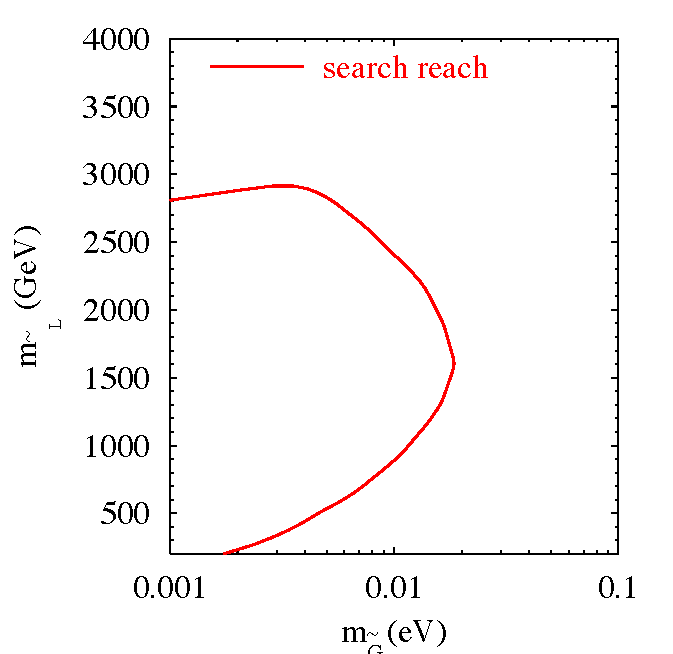
\includegraphics[width=5cm]{Fig1.pdf}
    \caption{...caption...}
    \label{fig:projname:plot1}
  \end{center}
\end{figure}
%% ~\newline~
%% To reference the main parts of the documents, use standard latex commands, with a prefix sec: and cha:.
%%
%% Examples: cha:nnlo will point to Chapter~\ref{cha:nnlo}.
%% Most likely, the conveners will fix these references at the end.
\end{itemize}
~\newline~
To use macros, define them locally, but then un-define them at the end of your local tex file.

Examples `` \Herwig{} `` is written using a macro, which is defined
in the local tex file, and undefined at the end of it.

\subsection{you can write subsections...}
Example of citation: in Ref.~\cite{Belanger:2014vza}

\subsubsection{and subsubsections...}

%= undefine macros (MANDATORY) ====================
\let\Herwig\undefined
\let\Pythia\undefined
\let\Sherpa\undefined
\let\Rivet\undefined
\let\Professor\undefined
\let\eps\undefined
\let\mc\undefined
\let\mr\undefined
\let\mb\undefined
\let\tm\undefined




